\documentclass[10pt]{book}

\usepackage{cdtBook}
\usepackage{usecases}
\usepackage{txfonts}
\title{Trabajo terminal\bigskip\\Videojuego Yolotl}
\subtitle{Componente 2 Iteración 2 Especificación del proyecto}
\author{Nombre del equipo o consultoría}
\organization{Escuela Superior de Cómputo, IPN}
\showInstrucciones
\date{\color{red}Borrador del 21 de febrero del 2017\\(para revisión)}
%\date{\color{green}Version 1.0}

%%%%%%%%%%%%%%%%%%%%%%%%%%%%%%%%%%%%%%%%%%%%%%%%%%%%%%%%%%%%%%%%
\begin{document}

\ThisLRCornerWallPaper{1}{images/bannerAzul}
\maketitle
\thispagestyle{empty}


\frontmatter
\tableofcontents
\listoffigures
\listoftables


%=========================================================
%\chapter{Project Charter}

\newcommand{\ESCOMPchSec}[1]{\rowcolor{colorAgua}\multicolumn{4}{|c|}{\bf #1}\\\hline}
\newcommand{\ESCOMPchItem}[2]{{\bf {#1}} & \multicolumn{3}{p{.66\textwidth}|}{#2}\\\hline}
\newcommand{\ESCOMPchSubItem}[3]{{\bf {#1}} & {#2} & \multicolumn{2}{p{.44\textwidth}|}{#3}\\\hline}
\newcommand{\ESCOMPchSubSubItem}[4]{{\bf {#1}} & {#2} & {#3}& {#4}\\\hline}

\cleardoublepage
{\centering{\Huge Project Charter}\bigskip\\}
\begin{table}[hptb!] 
%\renewcommand\thetable{i}
\begin{tabular}{|p{.22\textwidth} |p{.22\textwidth} |p{.22\textwidth} |p{.22\textwidth} |}
	\hline
	\ESCOMPchItem{Proyecto:}{CVE, Nombre proyecto.}
	\ESCOMPchItem{Responsable:}{Empresa, Nombre del responsable, cargo, Firma.}
	\ESCOMPchItem{Autoriza:}{Empresa, Nombre del responsable, cargo, Firma.}
	\ESCOMPchItem{Background/Contexto:}{Descripción breve del contexto, no mas de 3 líneas.}
	\ESCOMPchItem{Beneficios esperados:}{Principales beneficios al término del proyecto.}
	\ESCOMPchItem{Costo estimado:}{\$ 2,350,700.00 $\pm$ 13\% (por ejemplo.)}
	\ESCOMPchSubSubItem{Fecha de inicio:}{Fecha}{\bf Fecha de término:}{Fecha.}
	\ESCOMPchItem{Objetivo:}{Objetivo general del proyecto.}
	\ESCOMPchSec{Entregables Principales}
	\ESCOMPchSubItem{}{Clave-Nombre}{descripción del entregable}
	\ESCOMPchSubItem{}{Clave-Nombre}{descripción del entregable}
	\ESCOMPchSubItem{}{...}{}
	\ESCOMPchSec{Alcance del proyecto}
	\ESCOMPchItem{Incluye:}{
		\begin{Titemize}
			\Titem Elemento 1 del alcance que incluye.
			\Titem ...
		\end{Titemize}
	}
	\ESCOMPchItem{Excluye:}{
		\begin{Titemize}
			\Titem Elemento 1 del alcance que incluye.
			\Titem ...
		\end{Titemize}
	}
	\ESCOMPchItem{Criterio de éxito:}{Indicador clave de término del proyecto}
	\ESCOMPchItem{Metodología:}{Metodología o metodologías que se utilizan (dos renglones o lista de no mas de 7)}
	\ESCOMPchSec{Datos de contacto}
	\ESCOMPchItem{Project Manager:}{Nombre, Tel, correo, etc.}
	\ESCOMPchItem{Project owner:}{Nombre, Tel, correo, etc.}
	\ESCOMPchItem{...}{}
	\ESCOMPchItem{Riesgos y peligros:}{
		\begin{Titemize}
			\Titem Riesgo o peligro identificado.
			\Titem ...
		\end{Titemize}
	}
	\ESCOMPchItem{Supuestos:}{
		\begin{Titemize}
			\Titem Suposiciones hechas de las que depende el éxito del proyecto.
			\Titem ...
		\end{Titemize}
	}
	\ESCOMPchItem{Restricciones y dependencias:}{
		\begin{Titemize}
			\Titem Restricciones del proyecto.
			\Titem ...
		\end{Titemize}
	}
	\ESCOMPchSec{Supervisión}
	\ESCOMPchSubItem{Juntas:}{(Nombre de la(s) persona(s)),}{ reporta a (Nombre de la(s) persona(s))}
	\ESCOMPchSubItem{Dudas:}{(Nombre de la(s) persona(s)),}{ reporta a (Nombre de la(s) persona(s))}
	\ESCOMPchSubItem{Avances:}{(Nombre de la(s) persona(s)),}{ reporta a (Nombre de la(s) persona(s))}
	\ESCOMPchSubItem{...}{}{}
\end{tabular}
	\caption{Resumen del proyecto}
	\label{tbl:projectCharter}
\end{table}


\mainmatter
\LRCornerWallPaper{1}{images/plecaAyD}

%%%%%%%%%%%%%%%%%%%%%%%%%%%%%%%%%%%%%%%%%%%%%%%%%%%%%%%%%%%%%%%%

%=========================================================
%oliwis aqui estoy
%escribiendo puras
%tonterias en este documento
%porque no se me ocurre otra cosa
%xD
%=========================================================
\chapter{Introducción}


\cdtInstrucciones{
	Presentar el documento, indicando su contenido, a quien va dirigido, quien lo realizó, por que razón, dónde y cuando. \\
}
	Este documento contiene la Especificacion del ptoyecto ``{\em Nombre del proyecto}'' correspondiente al trabajo realizado en el semestre 2016-2017-2 para la materia de Análisis y diseño orientado a objetos en el grupo 2CV9 por el equipo {\em Nombre del equipo}.

%---------------------------------------------------------
\section{Presentación}


\cdtInstrucciones{
	Indique el propósito del documento y las distintas formas en que puede ser utilizado.\\
}
	Este documento contiene la especificación de los requerimientos del usuario y del sistema del sistema a desarrollar. Tiene como objetivo establecer la naturaleza y funciones del sistema para su evaluación al final del semestre. Este documento debe ser aprobado por los principales responsables del proyecto.
	
	Este documento es el C2-EP1 del proyecto ``{\em Nombre del proyecto}''.
	
%---------------------------------------------------------
\section{Organización del contenido}

	En el capítulo \ref{cap:reqUsr} ...
	
	En el capítulo \ref{cap:reqSist} ...

%---------------------------------------------------------
\section{Notación, símbolos y convenciones utilizadas}

	Los requerimientos funcionales utilizan una clave RFX, donde:
	
\begin{description}
	\item[X] Es un número consecutivo: 1, 2, 3, ...
	\item[RF] Es la clave para todos los {\bf R}equerimientos {\bf F}uncionales.
\end{description}

	Los requerimientos del usuario utilizan una clave RUX, donde:
	
\begin{description}
	\item[X] Es un número consecutivo: 1, 2, 3, ...
	\item[RU] Es la clave para todos los {\bf R}equerimientos del {\bf U}suario.
\end{description}

	Además, para los requerimeitnos funcionales se usan las abreviaciones que se muestran en la tabla~\ref{tbl:leyendaRF}.
\begin{table}[hbtp!]
	\begin{center}
    \begin{tabular}{|r l|}
	    \hline
    	{\footnotesize Id} & {\footnotesize\em Identificador del requerimiento.}\\
    	{\footnotesize Pri.} & {\footnotesize\em Prioridad}\\
    	{\footnotesize Ref.} & {\footnotesize\em Referencia a los Requerimientos de usuario.}\\
    	{\footnotesize MA} & {\footnotesize\em Prioridad Muy Alta.}\\
    	{\footnotesize A} & {\footnotesize\em Prioridad Alta.}\\
    	{\footnotesize M} & {\footnotesize\em Prioridad Media.}\\
    	{\footnotesize B} & {\footnotesize\em Prioridad Baja.}\\
    	{\footnotesize MB} & {\footnotesize\em Prioridad Muy Baja.}\\
		\hline
    \end{tabular} 
    \caption{Leyenda para los requerimientos funcionales.}
    \label{tbl:leyendaRF}
	\end{center}
\end{table}

%=========================================================
%=========================================================
\chapter{Modelo del Alcance}
\label{cap:reqUsr}

	En este capítulo se modela el alcance del sistema. Se presentan inicialmente los Actores involucrados y sus requerimientos, especificando cuales se alcanzaron en la primera iteración y cuales serán trabajados en la segunda iteración. Después se presentan los requerimientos funcionales de esta iteración y al final se presenta el modelo Físico y Lógico del sistema.


%---------------------------------------------------------
\section{Modelado de Usuarios}
\cdtInstrucciones{
	Identifique los actores que estarán involucrados en los procesos relacionados con el sistema para esta iteración de desarrollo. Ponga énfasis en los procesos involucrados.
}

\subsection{Organigrama de la Empresa}

	

\begin{figure}[htbp]
	\begin{center}
		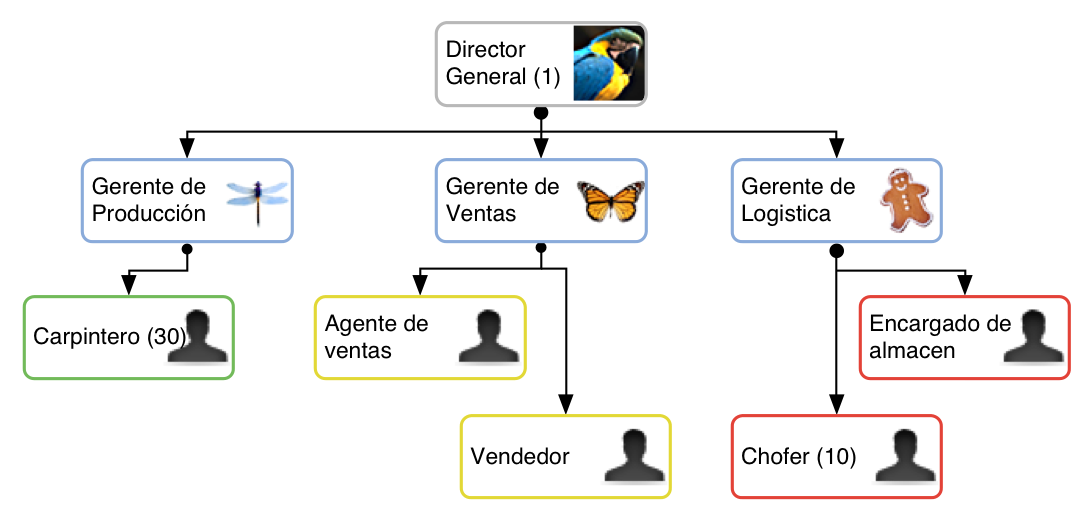
\includegraphics[width=.8\textwidth]{images/organigramaEm}
		\caption{Organigrama de la Mueblería Qetzal S. A. de C. V.}
		\label{fig:organigrama}
	\end{center}
\end{figure}


%---------------------------------------------------------
\begin{Usuario}{\subsection{Gerente de Ventas}}{
	Es el encargado de todas las operaciones de ventas al mayoreo y al menudeo. coordina y supervisa el trabajo de los Agentes de Ventas y Encargados de Tienda.
	Reporta directamente al Gerente de Operaciones
}
    \item[Responsabilidades:] \cdtEmpty
    \begin{itemize}
		\item Supervisar la operación de ventas.
		\item Plantear y supervisar el logro de las metas de ventas de la empresa y su crecimiento económico.
		\item ...
    \end{itemize}

	\item[Perfil:] \cdtEmpty
    \begin{itemize}
		\item Amplia experiencia en el ramo.
		\item Licenciatura como mínimo.
		\item ...
    \end{itemize}
	\item[Procesos en los que participa:] \cdtEmpty
    \begin{itemize}
		\item PC-V01 Aprobar las ordenes de compra al mayoreo.
		\item PC-V02 Supervisar las ventas al menudeo.
		\item PC-V03 Elaborar informe de ventas mensual.
		\item ...
    \end{itemize}
\end{Usuario}

%---------------------------------------------------------
\begin{Usuario}{\subsection{Agente de Ventas}}{
	...
}
    \item[Responsabilidades:] \cdtEmpty
    \begin{itemize}
		\item ...
    \end{itemize}

	\item[Perfil:] \cdtEmpty
    \begin{itemize}
		\item ...
    \end{itemize}
	\item[Procesos en los que participa:] \cdtEmpty
    \begin{itemize}
		\item PC-V08 Venta al Mayoreo.
		\item ...
    \end{itemize}
\end{Usuario}


%---------------------------------------------------------
\section{Requerimientos de usuario}

\cdtInstrucciones{
	Identifique y describa los requerimientos funcionales del sistema señalando: id, nombre, descripción y prioridad.
}

\begin{table}[htbp!]
	\begin{requerimientosU}
		\FRitem{RU1}{Control de vehículos}{El usuario requiere llevar un registro actualizado de los vehículos, sus características y su estado.}{1}{\DONE}
		\FRitem{RU2}{Registro de ventas}{El usuario requiere llevar un registro actualizado de todas las ventas realizadas por mes y su status: pedido, entregado, pagado, etc..}{2}{\TODO}
		\FRitem{RU3}{Registro de clientes}{El usuario requiere llevar un registro actualizado de todos los clientes para su seguimiento, atención y tareas de promoción y mercadotecnia.}{1}{\DONE}
		\FRitem{RU4}{Planeación de entregas}{El usuario requiere una herramienta que le facilite la planeación de vehículos para que esta sea la más adecuada.}{-}{\PLAN}
		\FRitem{...}{...}{...}{...}{...}
	\end{requerimientosU}
    \caption{Requerimientos funcionales del sistema.}
    {\footnotesize\em Para leer correctamente esta tabla vea la leyenda en la Tabla~\ref{tbl:leyendaRF} en la página~\pageref{tbl:leyendaRF}.}
    \label{tbl:reqFunc}
\end{table}



%---------------------------------------------------------
\section{Especificación de plataforma}	

\cdtInstrucciones{
	Coloque un diagrama y su descripción para aclarar el tipo de solución propuesta. \\
	
 En esta sección se debe aclarar:
	
\begin{description}
	\item[Tipo de sistema:] Web, aplicación móvil, de escritorio, híbrida, etc.
	\item[Software requerido:] Programas que se deberán instalar, desde el sistema operativo, compiladores, interpretes, servidores, etc.
	\item[Hardware requerido:] CPU, núcleos, velocidad, memoria, disco duro, etc.
	\item[servicios:] De conexión, seguridad, firewall, respaldo de energía, redundancia, uso de raids, etc.
\end{description}
}

\begin{figure}[htbp!]
	\begin{center}
		\fbox{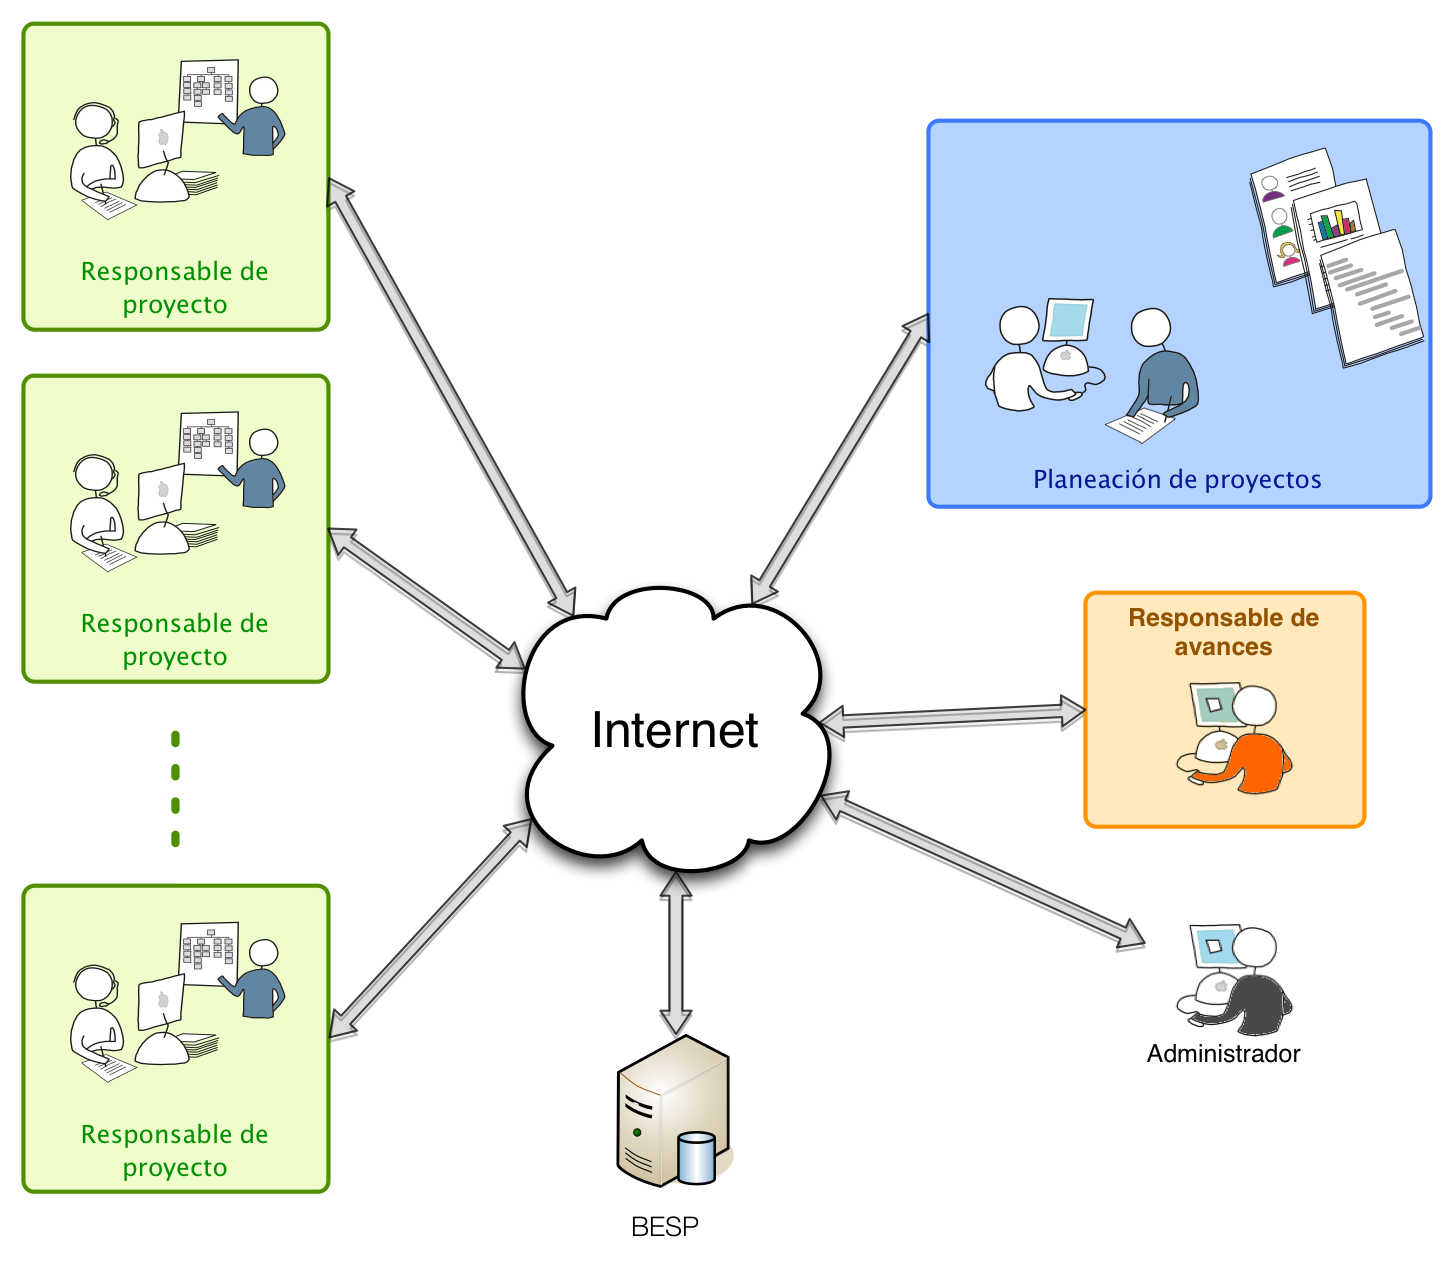
\includegraphics[width=.6\textwidth]{images/arquitectura}}
		\caption{Arquitectura del sistema.}
		\label{fig:arquitectura}
	\end{center}
\end{figure}

En la figura~\ref{fig:arquitectura} se describe la estructura del sistema, en ella se detalla ...




%=========================================================
%=========================================================
\chapter{Modelo del Negocio}	
\label{cap:reqSist}

	En este capítulo se modela la {\em Arquitectura del negocio} la cual está conformada por la Ontología del negocio ({\em Términos} y {\em Hechos del negocio}), Arquitectura de procesos y las {\em Reglas del negocio}. Primero se especifica brevemente el {\em Contexto} en el que los términos tienen significado.
	
	En las secciones \ref{sec:terminosDeNegocio} y \ref{sec:hechosDeNegocio} se presentan los Términos del negocio a manera de Glosario y por último se presentan los Hechos del negocio a manera de relaciones entre términos del negocio.

%----------------------------------------------------------
\section{Contexto}

	\cdtInstrucciones{El contexto debe explicar bajo que ambiente los términos del negocio son aplicables y proporcionar información general para su comprensión inicial.\\}
	La empresa ``Fast Rent'' se dedica a la renta de vehículos automotores, principalmente automóviles y motocicletas. Los clientes rentan vehículos por tiempos determinados y la empresa se encarga de dar mantenimiento a los vehículos y administrarlos para que estén disponibles para sus clientes. Los empleados, se dedican a labores de gerencia, atención a clientes, mantenimiento y soporte para los vehículos activos.
	
%---------------------------------------------------------
\section{Términos del Negocio}
\label{sec:terminosDeNegocio}

\begin{description}
	% Ejemplo de un término literal.
	\item[\hypertarget{tAutomovil}{Automóvil:}] ({\em es un tipo de \hyperlink{tVehiculo}{Vehículo}}) De cuatro ruedas con capacidad de 5 a 9 personas. 
	% Ejemplo de un término de entidad
	\item[\hypertarget{tCliente}{Cliente:}] Se refiere a todas las personas físicas y morales que \hyperlink{tRenta}{rentan} o han rentado un \hyperlink{tVehiculo}{vehículo}.
	
	\item[\hypertarget{tDirector}{Director:}] ({\em es un tipo de \hyperlink{tEmpleado}{Empleado}}) Es el empleado que tiene mayor rango de todos y no tiene superior, a diferencia de los demás.	
	\item[\hypertarget{tEmpleado}{Empleado:}] Se refiere a cualquier persona que labore en la empresa.
	
	\item[\hypertarget{tChecador}{Checador:}] ({\em Reloj asociado al atributo:} Hora de entrada y salida de un \hyperlink{tEmpleado}{empleado}. {\em Frecuencia de lectura:} Una vez al día para la entrada y otra para la salida durante los días laborales.
	
	\item[\hypertarget{tMotocicleta}{Motocicleta:}] ({\em es un tipo de {tVehiculo}{Vehículo}}) De dos ruedas con capacidad para una personas. 

	\item[\hypertarget{tRenta}{Renta:}] Se refiere al servicio que ofrece la empresa para prestar \hyperlink{tVehiculo}{vehículos} a los \hyperlink{tCliente}{clientes} por un tiempo definido.
	
	\item[\hypertarget{tVehiculo}{Vehiculo:}] Se refiere a los automóviles y motocicletas que la empresa usa para dar el servicio de renta a los \hyperlink{tCliente}{clientes}.
	
%	\brTermSensor{tVelocimetro}{Velocímetro:}{Velocidad de un Vehículo.}{Kilometros/hora.}{Constantemente siempre que el \cdtRef{tVehiculo}{vehículo} esté encendido.}
\end{description}

%----------------------------------------------------------
\section{Modelo del dominio del problema}
\label{sec:hechosDeNegocio}


%- - - - - - - - - - - - - - - - - - - - - - - - - - - - - 
\subsection{Modelo del dominio del problema}

	El modelo del dominio del problema se muestra en la figura~\ref{fig:modeloDeDominio}, a continuación se describen cada una de las entidades y sus relaciones.
	
\begin{figure}[htbp!]
	\begin{center}
		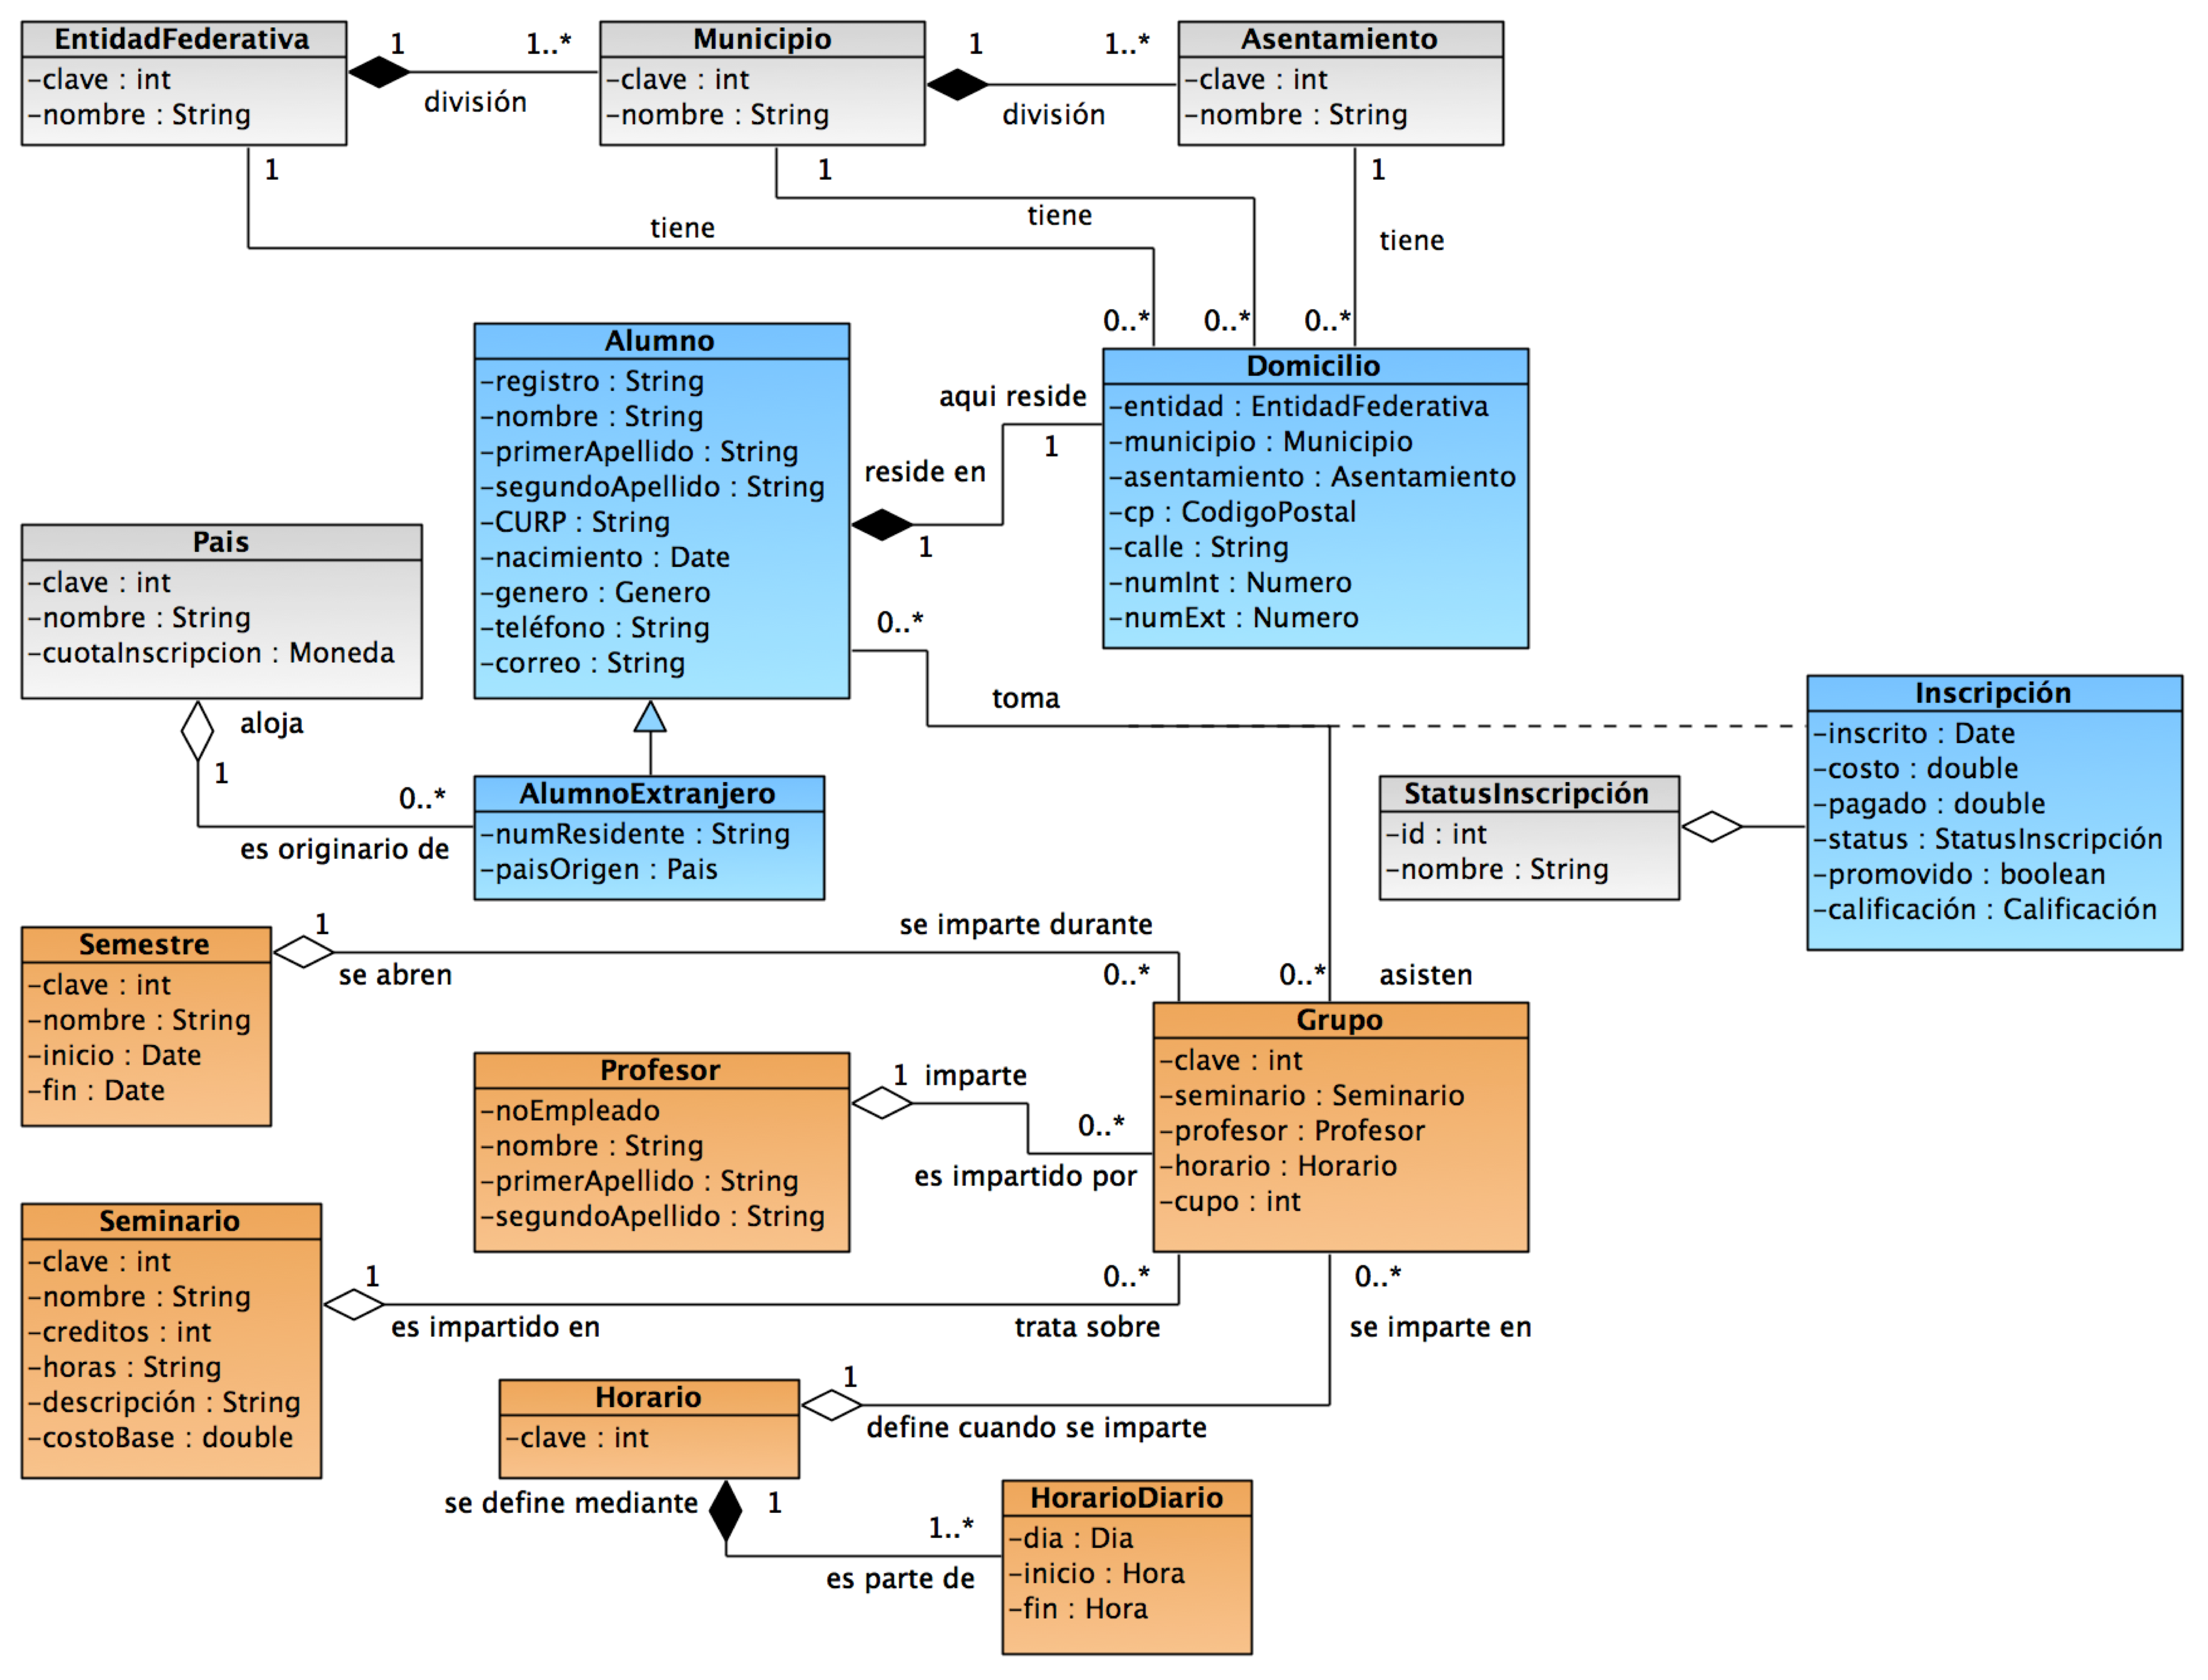
\includegraphics[angle=90,width=.95\textwidth]{images/modeloDelDominioDelProblema}
		\caption{Modelo del dominio del problema}
		\label{fig:modeloDeDominio}
	\end{center}
\end{figure}

%- - - - - - - - - - - - - - - - - - - - - - - - - - - - - 

\newenvironment{cdtEntidad}[2]{%
	\def \varBusinessEntityId{#2}%
	\hypertarget{#1}{\hspace{1pt}}%
	\newline%
	\noindent{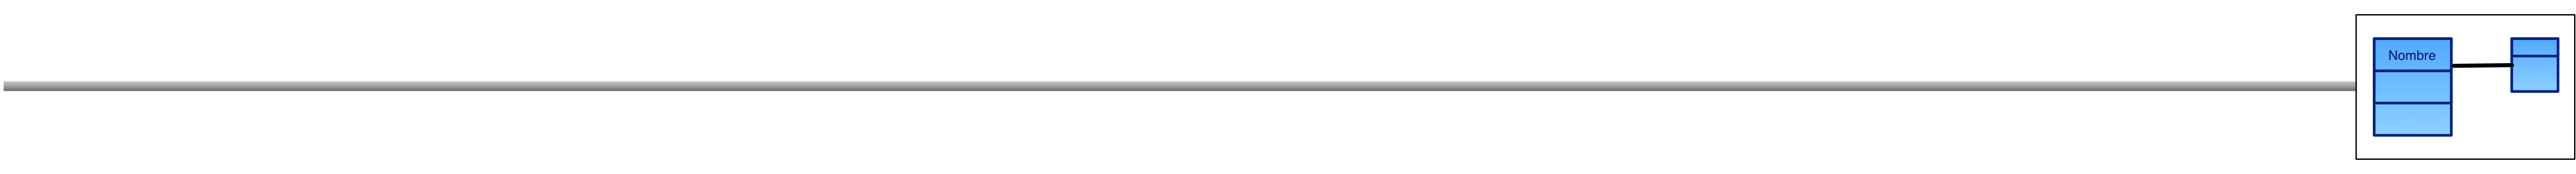
\includegraphics[width=\textwidth]{images/uc/classRule}}%
	\vspace{-25pt}%
	\subsection{Entidad: #2}%
	\noindent\begin{longtable}{|p{.2\textwidth}| p{.15\textwidth} | p{.46\textwidth} |p{.08\textwidth} |}%
	\hline%
	\multicolumn{4}{|c|}{{\cellcolor{colorSecundario}\color{white}Atributos}}\\ \hline%
	{\cellcolor{colorAgua}Nombre} &%
	{\cellcolor{colorAgua}Tipo} &%
	{\cellcolor{colorAgua}Descripción} &%
	{\cellcolor{colorAgua}Requerido}%
	\\ \hline%
	\endhead%
}{%
	\end{longtable}%
}

\newcommand{\brAttr}[5]{%
	{\bf\hypertarget{\varBusinessEntityId:#1}{#2}} & {\em{#3}} & {#4} & #5 \\\hline
}

\newcommand{\cdtEntityRelSection}{%
	\multicolumn{4}{|c|}{{\cellcolor{colorSecundario}\color{white}Relaciones}}\\ \hline%
	{\cellcolor{colorAgua}Tipo de relación} &%
	{\cellcolor{colorAgua}Entidad} &%
	\multicolumn{2}{|c|}{{\cellcolor{colorAgua}Rol}}
	\\ \hline%
}

\newcommand{\brRelComposition}{{\color{colorPrincipal}$\Diamondblack$\hspace{-1pt}---Composición}}
\newcommand{\brRelAgregation}{{\color{colorPrincipal}$\Diamond$\hspace{-1pt}---Agregación}}
\newcommand{\brRelGeneralization}{{\color{colorPrincipal}$\lhd$\hspace{-1pt}---Generalización}}

\newcommand{\brRel}[3]{%
	{\em{#1}} & {\bf{#2}} & \multicolumn{2}{|l|}{#3}\\\hline
}


%- - - - - - - - - - - - - - - - - - - - - - - - - - - - - 
\begin{cdtEntidad}{Alumno}{Alumno}
	\brAttr{registro}{Registro}{Id}{Número de registro utilizado para identificar un alumno}{Sí}
	\brAttr{nombre}{Nombre}{Palabra Corta}
		{Nombre o nombres del alumno.}{Sí}
	\brAttr{primerApellido}{Primer apellido}{Palabra Corta}
		{Primer apellido del alumno.}{Sí}
	\brAttr{segundoApellido}{Segundo apellido}{Palabra Corta}
		{Segundo apellido del alumno.}{No}
	\brAttr{CURP}{CURP}{CURP}
		{CURP del alumno.}{Sí}
	\brAttr{nacimiento}{Nacimiento}{Fecha}
		{Fecha de nacimiento del alumno.}{Sí}
	\brAttr{genero}{Género}{Domicilio}
		{Género del alumno.}{No}
	\brAttr{telefono}{Teléfono}{Telefono}
		{Teléfono para contactar al alumno.}{Sí}
	\brAttr{correo}{Correo}{Correo}
		{Correo del alumno para enviar información académica y escolar y para recuperación de clave de acceso.}{Sí}
	\cdtEntityRelSection
	\brRel{\brRelComposition}{Domicilio}{Un \hyperlink{Alumno}{Alumno} reside en un \hyperlink{Domicilio}{Domicilio}}	
	\brRel{\brRelAgregation}{Grupo}{Un \hyperlink{Alumno}{Alumno} toma un \hyperlink{Curso}{Curso}}	
\end{cdtEntidad}

%- - - - - - - - - - - - - - - - - - - - - - - - - - - - - 
\begin{cdtEntidad}{AlumnoExtranjero}{Alumno Extranjero}%{}
	\brAttr{numeroResidente}{Numero de residente}{Id}{Número de registro dado por la Secretaría de Relaciones Exteriores a los extranjeros.}{Si}
	\brAttr{paisOrigen}{Pais origen}{\hyperlink{Pais}{País}}
		{País de origen del alumno extranjero.}{Sí}
	\cdtEntityRelSection
	\brRel{\brRelAgregation}{País}{Un \hyperlink{Alumno}{Alumno} es originario de un \hyperlink{Pais}{Pais}}	
	\brRel{\brRelGeneralization}{Alumno}{Un \hyperlink{AlumnoExtranjero}{Alumno Extranjero} es un  \hyperlink{Alumno}{Alumno}}	
\end{cdtEntidad}

%---------------------------------------------------------
\section{Modelado de Reglas de negocio}

\begin{BussinesRule}{BR8}{Fecha de Nacimiento correcta.}
	\BRitem[Tipo:] Regla de integridad referencial o estructural. 
				% Otras opciones para tipo: 
				% - Regla de integridad referencial o estructural. 
				% - Regla de operación, (calcular o determinar un valor.).
				% - Regla de inferencia de un hecho.
	\BRitem[Clase:] Habilitadora. 
				% Otras opciones para clase: Habilitadora, Cronometrada, Ejecutive.
	\BRitem[Nivel:] Control. % Otras opciones para nivel: Control, Influencia.
	\BRitem[Descripción:]	Las Fechas de Nacimiento que se registran en el SINACEM para cualquier Persona debe ser mayores al día Primero de Enero del año 1900 y menor a la Fecha Actual.
	\BRitem[Motivación:] Evitar fraudes al PRONIM por el registro de personas que no han nacido al momento de su registro.
	\BRitem[Sentencia:] $\forall p \in Persona \Rightarrow 01-Enero-1900~<~p.fechaDeNacimiento~<~fechaActual$.
	\BRitem[Ejemplo positivo:] Para el día 12 de Octubre del 2013, cumplen la regla: 		
        \begin{itemize}
        	\item 11 de Octubre del 2013
			\item 20 de Diciembre del 2010
			\item 2 de Enero del 1900
        \end{itemize}
	
	\BRitem[Ejemplo negativo:] Para el día 12 de Octubre del 2013, no cumplen la 
		\begin{itemize}
        	\item 12 de Octubre del 2013
			\item 20 de Diciembre del 2014
			\item 1 de Enero del 1900
			\item 31 de Diciembre del 1899
        \end{itemize}
	
	\BRitem[Referenciado por:] \hyperlink{CUCE3.2}{CUCE3.2}, \hyperlink{CUCE3.3}{CUCE3.3}.
\end{BussinesRule}

\begin{BussinesRule}{BR129}{Determinar si un Estudiante puede inscribir Seminario.} 
	\BRitem[Tipo:] Regla de integridad referencial o estructural. 
				% Otras opciones para tipo: 
				% - Regla de integridad referencial o estructural. 
				% - Regla de operación, (calcular o determinar un valor.).
				% - Regla de inferencia de un hecho.
	\BRitem[Clase:] Habilitadora. 
				% Otras opciones para clase: Habilitadora, Cronometrada, Ejecutive.
	\BRitem[Nivel:] Control. % Otras opciones para nivel: Control, Influencia.
	\BRitem[Descripción:] Un Estudiante requere del 80\% de créditos para inscribirse a un Seminario y no haber cursado y reprobado otro seminario.
	\BRitem[Ejemplo positivo:] 
	
	\BRitem[Ejemplo negativo:] 
	
	\BRitem[Referenciado por:] 
\end{BussinesRule}

\begin{BussinesRule}{BR130}{Determinar si un Estudiante puede inscribirse en un Seminario}
	\BRitem[Tipo:] Regla de inferencia de un hecho.
				% Otras opciones para tipo: 
				% - Regla de integridad referencial o estructural. 
				% - Regla de operación, (calcular o determinar un valor.).
				% - Regla de inferencia de un hecho.
	\BRitem[Clase:] Habilitadora. 
				% Otras opciones para clase: Habilitadora, Cronometrada, Ejecutive.
	\BRitem[Nivel:] Control. % Otras opciones para nivel: Control, Influencia.
	\BRitem[Descripción:] El Estudiante debe pertenecer a la Carrera del Seminario y debe haber Cupo en el grupo del Seminario.
	\BRitem[Ejemplo positivo:] 
	
	\BRitem[Ejemplo negativo:] 
	
	\BRitem[Referenciado por:] 
\end{BussinesRule}

\begin{BussinesRule}{BR143}{Validar el horario del estudiante}
	\BRitem[Tipo:] Regla de operación, (calcular o determinar un valor.).
				% Otras opciones para tipo: 
				% - Regla de integridad referencial o estructural. 
				% - Regla de operación, (calcular o determinar un valor.).
				% - Regla de inferencia de un hecho.
	\BRitem[Clase:] Habilitadora. 
				% Otras opciones para clase: Habilitadora, Cronometrada, Ejecutive.
	\BRitem[Nivel:] Control. % Otras opciones para nivel: Control, Influencia.
	\BRitem[Descripción:] Las Materias y Seminarios inscritos por el alumno, en un periodo específico, no pueden impartirse en el mismo día de la semana en horas traslapadas.
	\BRitem[Ejemplo positivo:] 
	
	\BRitem[Ejemplo negativo:] 
	
	\BRitem[Referenciado por:] 
\end{BussinesRule}

\begin{BussinesRule}{BR180}{Calcular costos del Estudiante}
	\BRitem[Tipo:] Regla de operación, (calcular o determinar un valor.).
				% Otras opciones para tipo: 
				% - Regla de integridad referencial o estructural. 
				% - Regla de operación, (calcular o determinar un valor.).
				% - Regla de inferencia de un hecho.
	\BRitem[Clase:] Habilitadora. 
				% Otras opciones para clase: Habilitadora, Cronometrada, Ejecutive.
	\BRitem[Nivel:] Control. % Otras opciones para nivel: Control, Influencia.
	\BRitem[Descripción:] Los servicios se cobran de la siguiente forma:
		\begin{Citemize}
			\item {\em Estudiantes Regulares:} Se les Cobran todos los servicios al 100\% de su costo.
			\item {\em Estudiantes becados:} Se les otorga un 80\% de descuento en el costo de todos los servicios (antes del IVA).
			\item {\em Estudiantes extranjeros:} Se les cobran los servicios al 200\% del costo registrado.
		\end{Citemize}
	\BRitem[Sentencia:] $\forall~e~\in~\mathbb{E}\textrm{studiantes}~\land~\forall~s~\in \mathbb{S}\textrm{eminario}~\Rightarrow$
		\begin{displaymath}
			Costo(e,s) = \left\{ \begin{array}{ll}
			s.costo & , si~e.tipo = \textrm{Estudiante regular}\\
			{s.costo}\over{5} & , si~e.tipo = \textrm{Estudiante becado}\\
			s.costo \cdot 2 & , si~e.tipo = \textrm{Estudiante extranjero}
			\end{array} \right.
		\end{displaymath}
	\BRitem[Ejemplo positivo:] 
	
	\BRitem[Ejemplo negativo:] 
	
	\BRitem[Referenciado por:] 
\end{BussinesRule}

\begin{BussinesRule}{BR45}{Calcular impuestos por seminario}
	\BRitem[Tipo:] Regla de operación, (calcular o determinar un valor.).
				% Otras opciones para tipo: 
				% - Regla de integridad referencial o estructural. 
				% - Regla de operación, (calcular o determinar un valor.).
				% - Regla de inferencia de un hecho.
	\BRitem[Clase:] Habilitadora. 
				% Otras opciones para clase: Habilitadora, Cronometrada, Ejecutive.
	\BRitem[Nivel:] Control. % Otras opciones para nivel: Control, Influencia.
	\BRitem[Descripción:] Los impuestos corresponden al 16\% correspondientes al IVA.
	\BRitem[Sentencia:] $Impuesto(e, s) = Costo(e, s)\cdot0.16$.
	\BRitem[Ejemplo positivo:] 
	
	\BRitem[Ejemplo negativo:] 
	
	\BRitem[Referenciado por:] 
\end{BussinesRule}

\begin{BussinesRule}{BR100}{Recibo del Estudiante por inscripción a Seminario.}
	\BRitem[Tipo:] Regla de operación, (calcular o determinar un valor.).
				% Otras opciones para tipo: 
				% - Regla de integridad referencial o estructural. 
				% - Regla de operación, (calcular o determinar un valor.).
				% - Regla de inferencia de un hecho.
	\BRitem[Clase:] Habilitadora. 
				% Otras opciones para clase: Habilitadora, Cronometrada, Ejecutive.
	\BRitem[Nivel:] Control. % Otras opciones para nivel: Control, Influencia.
	\BRitem[Descripción:] El  Recibo del Estudiante debe mostrar el total del costo con el siguiente desglose:
		\begin{displaymath}\begin{array}{lr}
			Costo: & \$ XXX.XX\\
			Descuento~aplicado~(YY\%): & \$ XXX.XX\\
			Subtotal: & \$ XXX.XX\\
			IVA~(16\%): & \$ XXX.XX\\\hline
			Total: & \$ XXX.XX
		\end{array}\end{displaymath}
	\BRitem[Sentencia:] $CostoTotal = Costo(e, s) + Impuesto(e, s)$.
	\BRitem[Ejemplo positivo:] 
	
	\BRitem[Ejemplo negativo:] 
	
	\BRitem[Referenciado por:] 
\end{BussinesRule}



%---------------------------------------------------------
\section{Modelo de Procesos AS-IS}

En esta sección se describen los procesos a mejorar con el sistema.

% - - - - - - - - - - - - - - - - - - - - - - - - - - - - 
\subsection{PROC-01 Análisis de requerimientos}

\begin{figure}[htbp]
	\begin{center}
		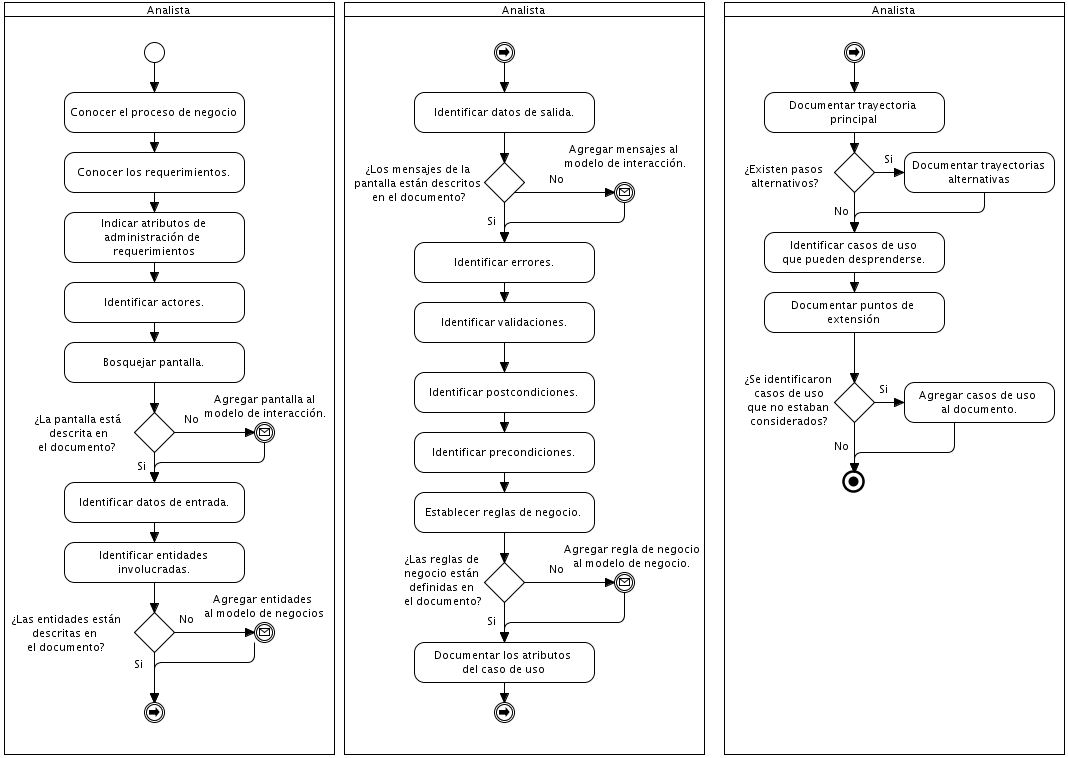
\includegraphics[width=.7\textwidth]{images/proceso1}
		\caption{PROC-01 Proceso de Análisis de requerimientos}
		\label{fig:proceso1}
	\end{center}
\end{figure}

\begin{description}
	\item[Descripción:] Describa el proceso indicando los aspectos relevantes que el diagrama no muestra.
	\item[Entradas:] \cdtEmpty
        \begin{itemize}
			\item Documentos de Procesos.
			\item Reglas de negocio.
			\item Minutas de las reuniones de análisis.
        \end{itemize}
	\item[Salidas:] \cdtEmpty
        \begin{itemize}
			\item Especificación de requerimientos.
			\item Bosquejo de pantallas.
			\item Modelo de base de datos
        \end{itemize}	
    \item[Áreas de oportunidad:] Liste los aspectos que detecta se pueden mejorar con la introducción del sistema o los problemas encontrados.
\end{description}

% - - - - - - - - - - - - - - - - - - - - - - - - - - - - 
\subsection{PROC-02 ...}

\begin{figure}[htbp]
	\begin{center}
		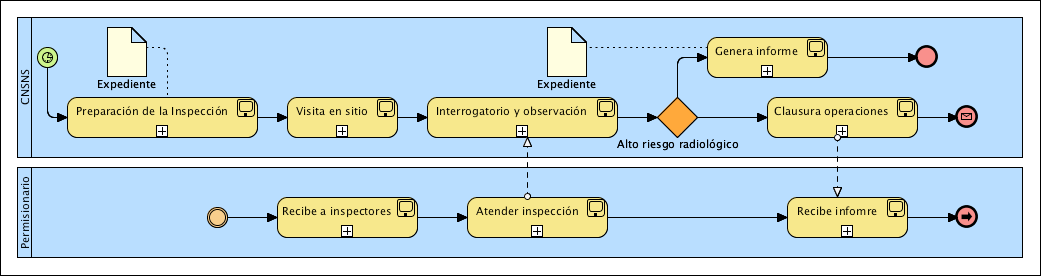
\includegraphics[width=.8\textwidth]{images/proceso2}
		\caption{PROC-02 Nombre del proceso}
		\label{fig:proceso2}
	\end{center}
\end{figure}

\begin{description}
	\item[Descripción:] ...
	\item[Entradas:] \cdtEmpty
        \begin{itemize}
			\item ...
        \end{itemize}
	\item[Salidas:] \cdtEmpty
        \begin{itemize}
			\item ...
        \end{itemize}	
    \item[Áreas de oportunidad:] Liste los aspectos que detecta se pueden mejorar con la introducción del sistema o los problemas encontrados.
\end{description}


%\input{proc/proc03.tex}
%\input{proc/proc04.tex}

%---------------------------------------------------------
\section{Modelo de procesos TO-BE}

Los nuevos procesos se presentan en esta sección, el mapa de procesos de se muestra en la figura~\ref{fig:mapaProc}.

\begin{figure}[htbp]
	\begin{center}
		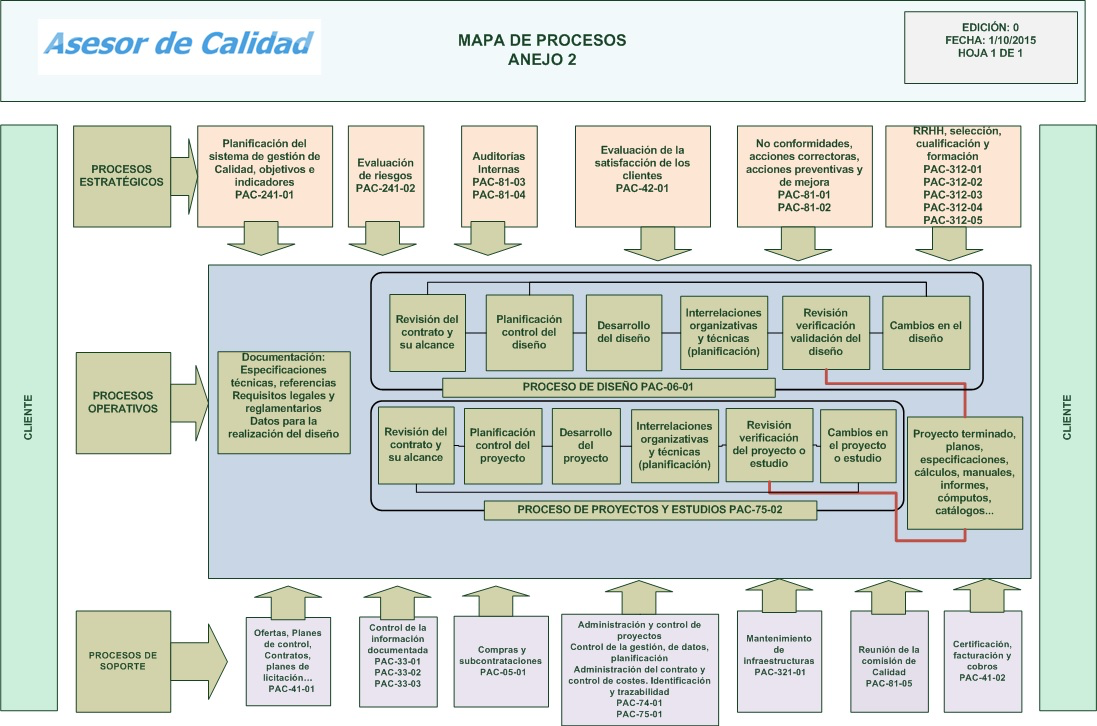
\includegraphics[width=.8\textwidth]{images/mapaProc}
		\caption{Mapa de procesos}
		\label{fig:mapaProc}
	\end{center}
\end{figure}


% - - - - - - - - - - - - - - - - - - - - - - - - - - - - 
\subsection{PROCM-01 ...}

\begin{figure}[htbp]
	\begin{center}
		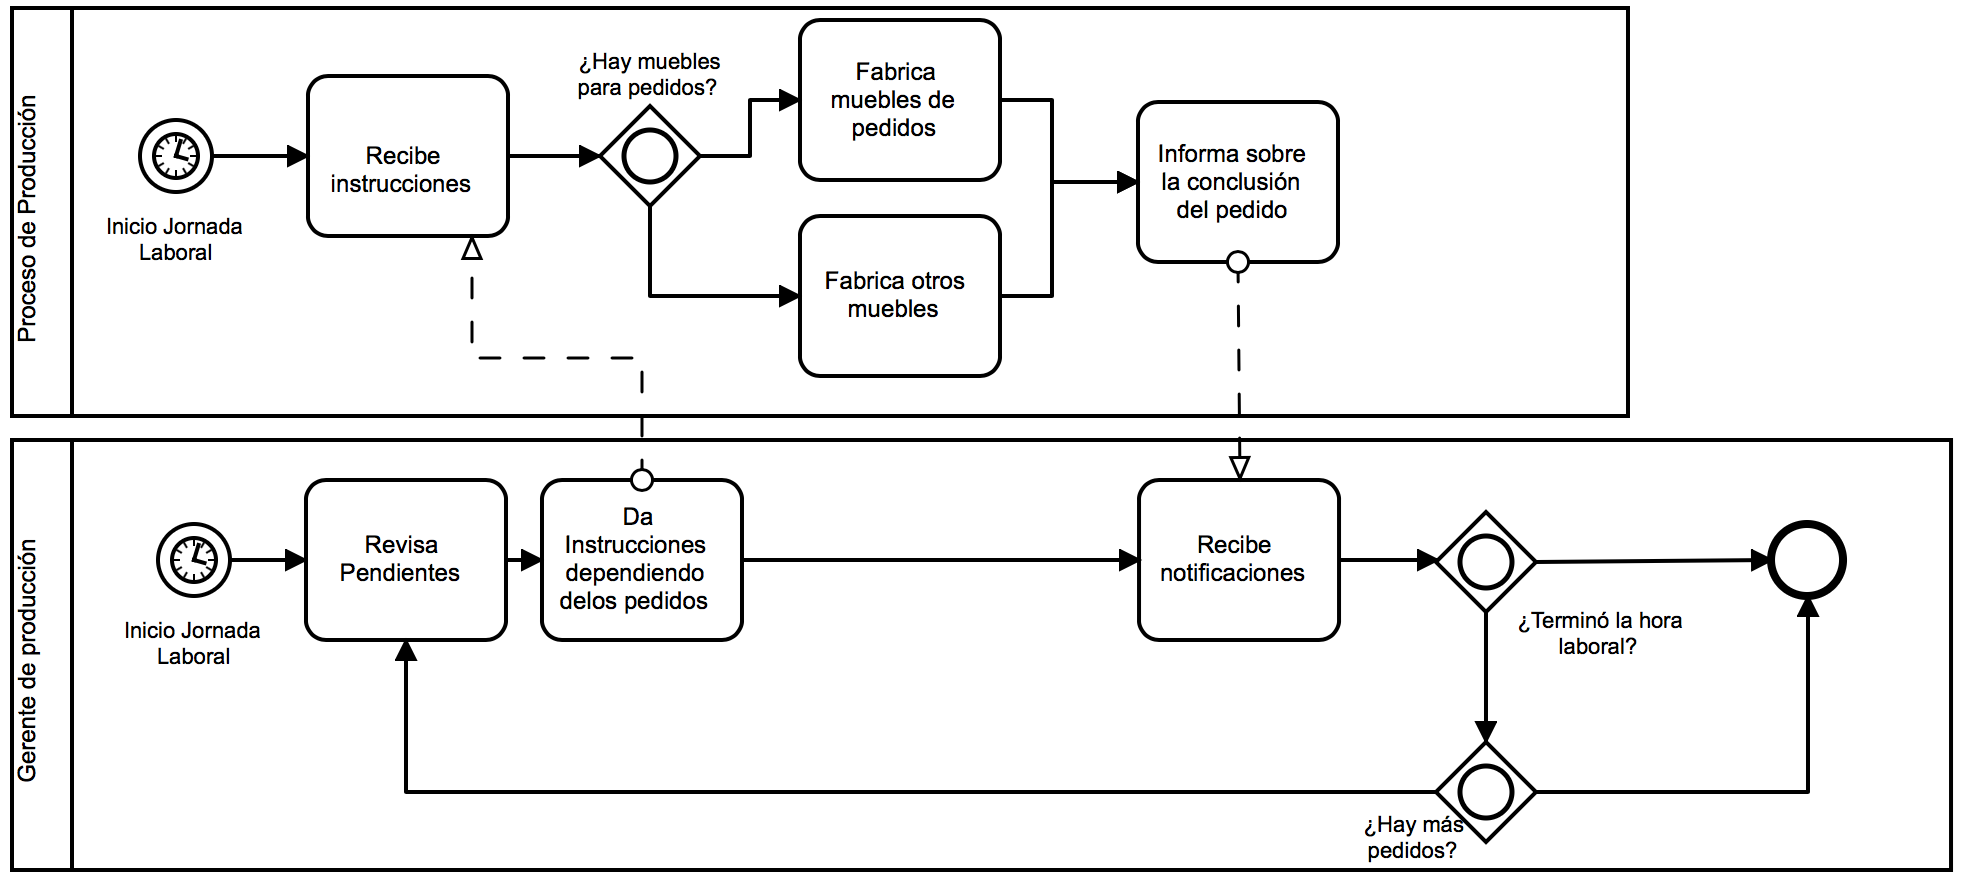
\includegraphics[width=.8\textwidth]{images/proceso3}
		\caption{PROCM-01 Nombre del proceso}
		\label{fig:proceso3}
	\end{center}
\end{figure}

\begin{description}
	\item[Descripción:] ...
	\item[Entradas:] \cdtEmpty
        \begin{itemize}
			\item ...
        \end{itemize}
	\item[Salidas:] \cdtEmpty
        \begin{itemize}
			\item ...
        \end{itemize}	
    \item[Mejoras esperadas:] Liste las mejoras que espera obtener tras la implementación del sistema.
    \item[Reglas de negocio:] \hyperlink{BR05}{BR05}, \hyperlink{BR8}{BR8}.
    \item[Casos de uso:] \hyperlink{CU3.4}{CU 3.4 Login}, \hyperlink{CU 4.3}{ CU 4.3 Consultar productos}.
\end{description}

%\input{proc/proc-m02.tex}
%\input{proc/proc-m03.tex}
%\input{proc/proc-m04.tex}



%=========================================================
%=========================================================
\chapter{Modelo dinámico}	
\label{cap:modDinamico}

	Este capítulo describe en modelo dinámico del sistema. en el se detallan todos los escenarios de ejecución del sistema. La figura~\ref{fig:casosDeUso} muestra el diagrama general del sistema y sus sib sistemas, y la figura~\ref{fig:casosDeUsoDetalle} muestra todos los casos de uso del sistema. En este documento solo detallamos los casos de uso del subsistema de gestión de cursos.
	
\begin{figure}[htbp]
	\begin{center}
		\fbox{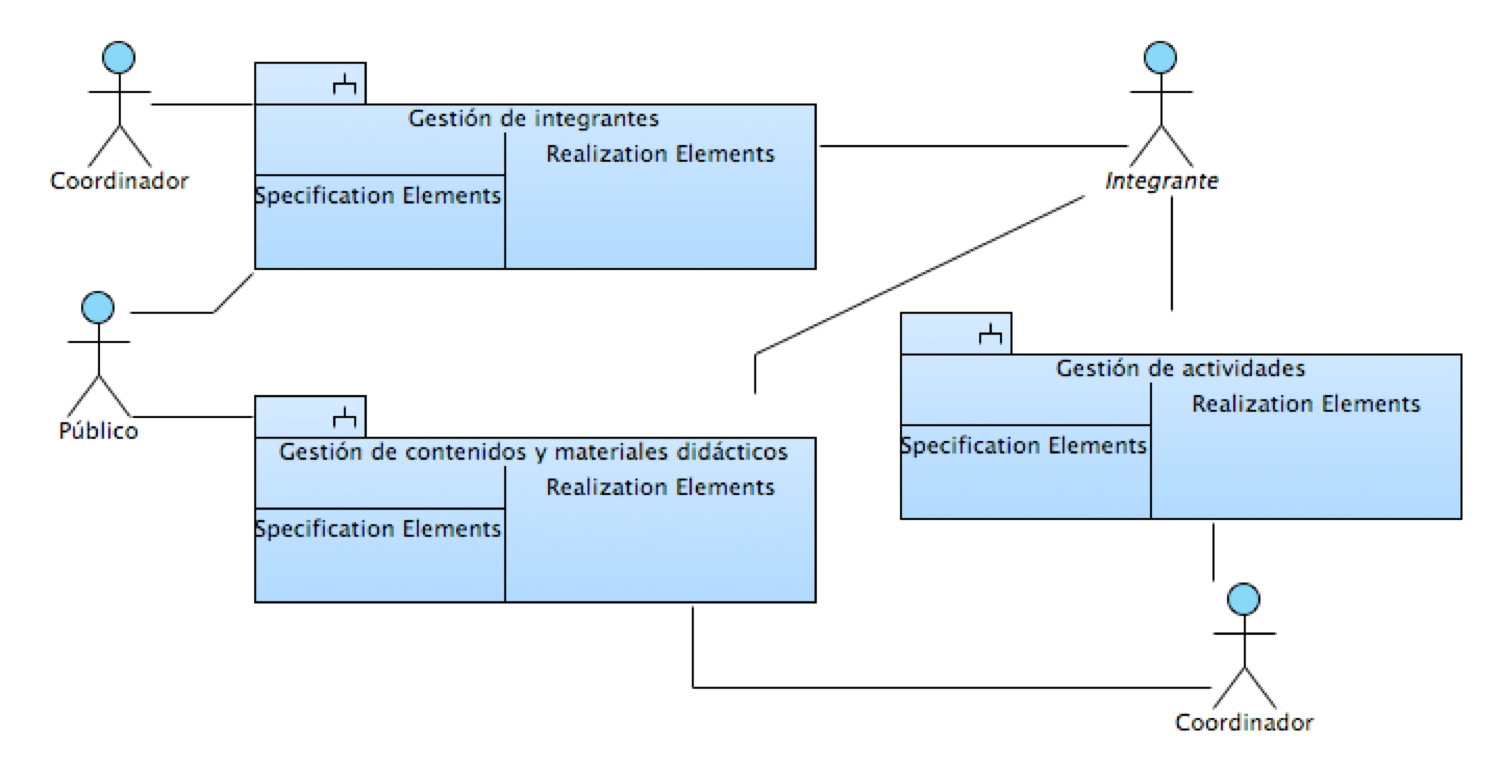
\includegraphics[width=.8\textwidth]{images/casosDeUso}}
		\caption{Diagrama de casos de uso del sistema.}
		\label{fig:casosDeUso}
	\end{center}
\end{figure}

\begin{figure}[htbp]
	\begin{center}
		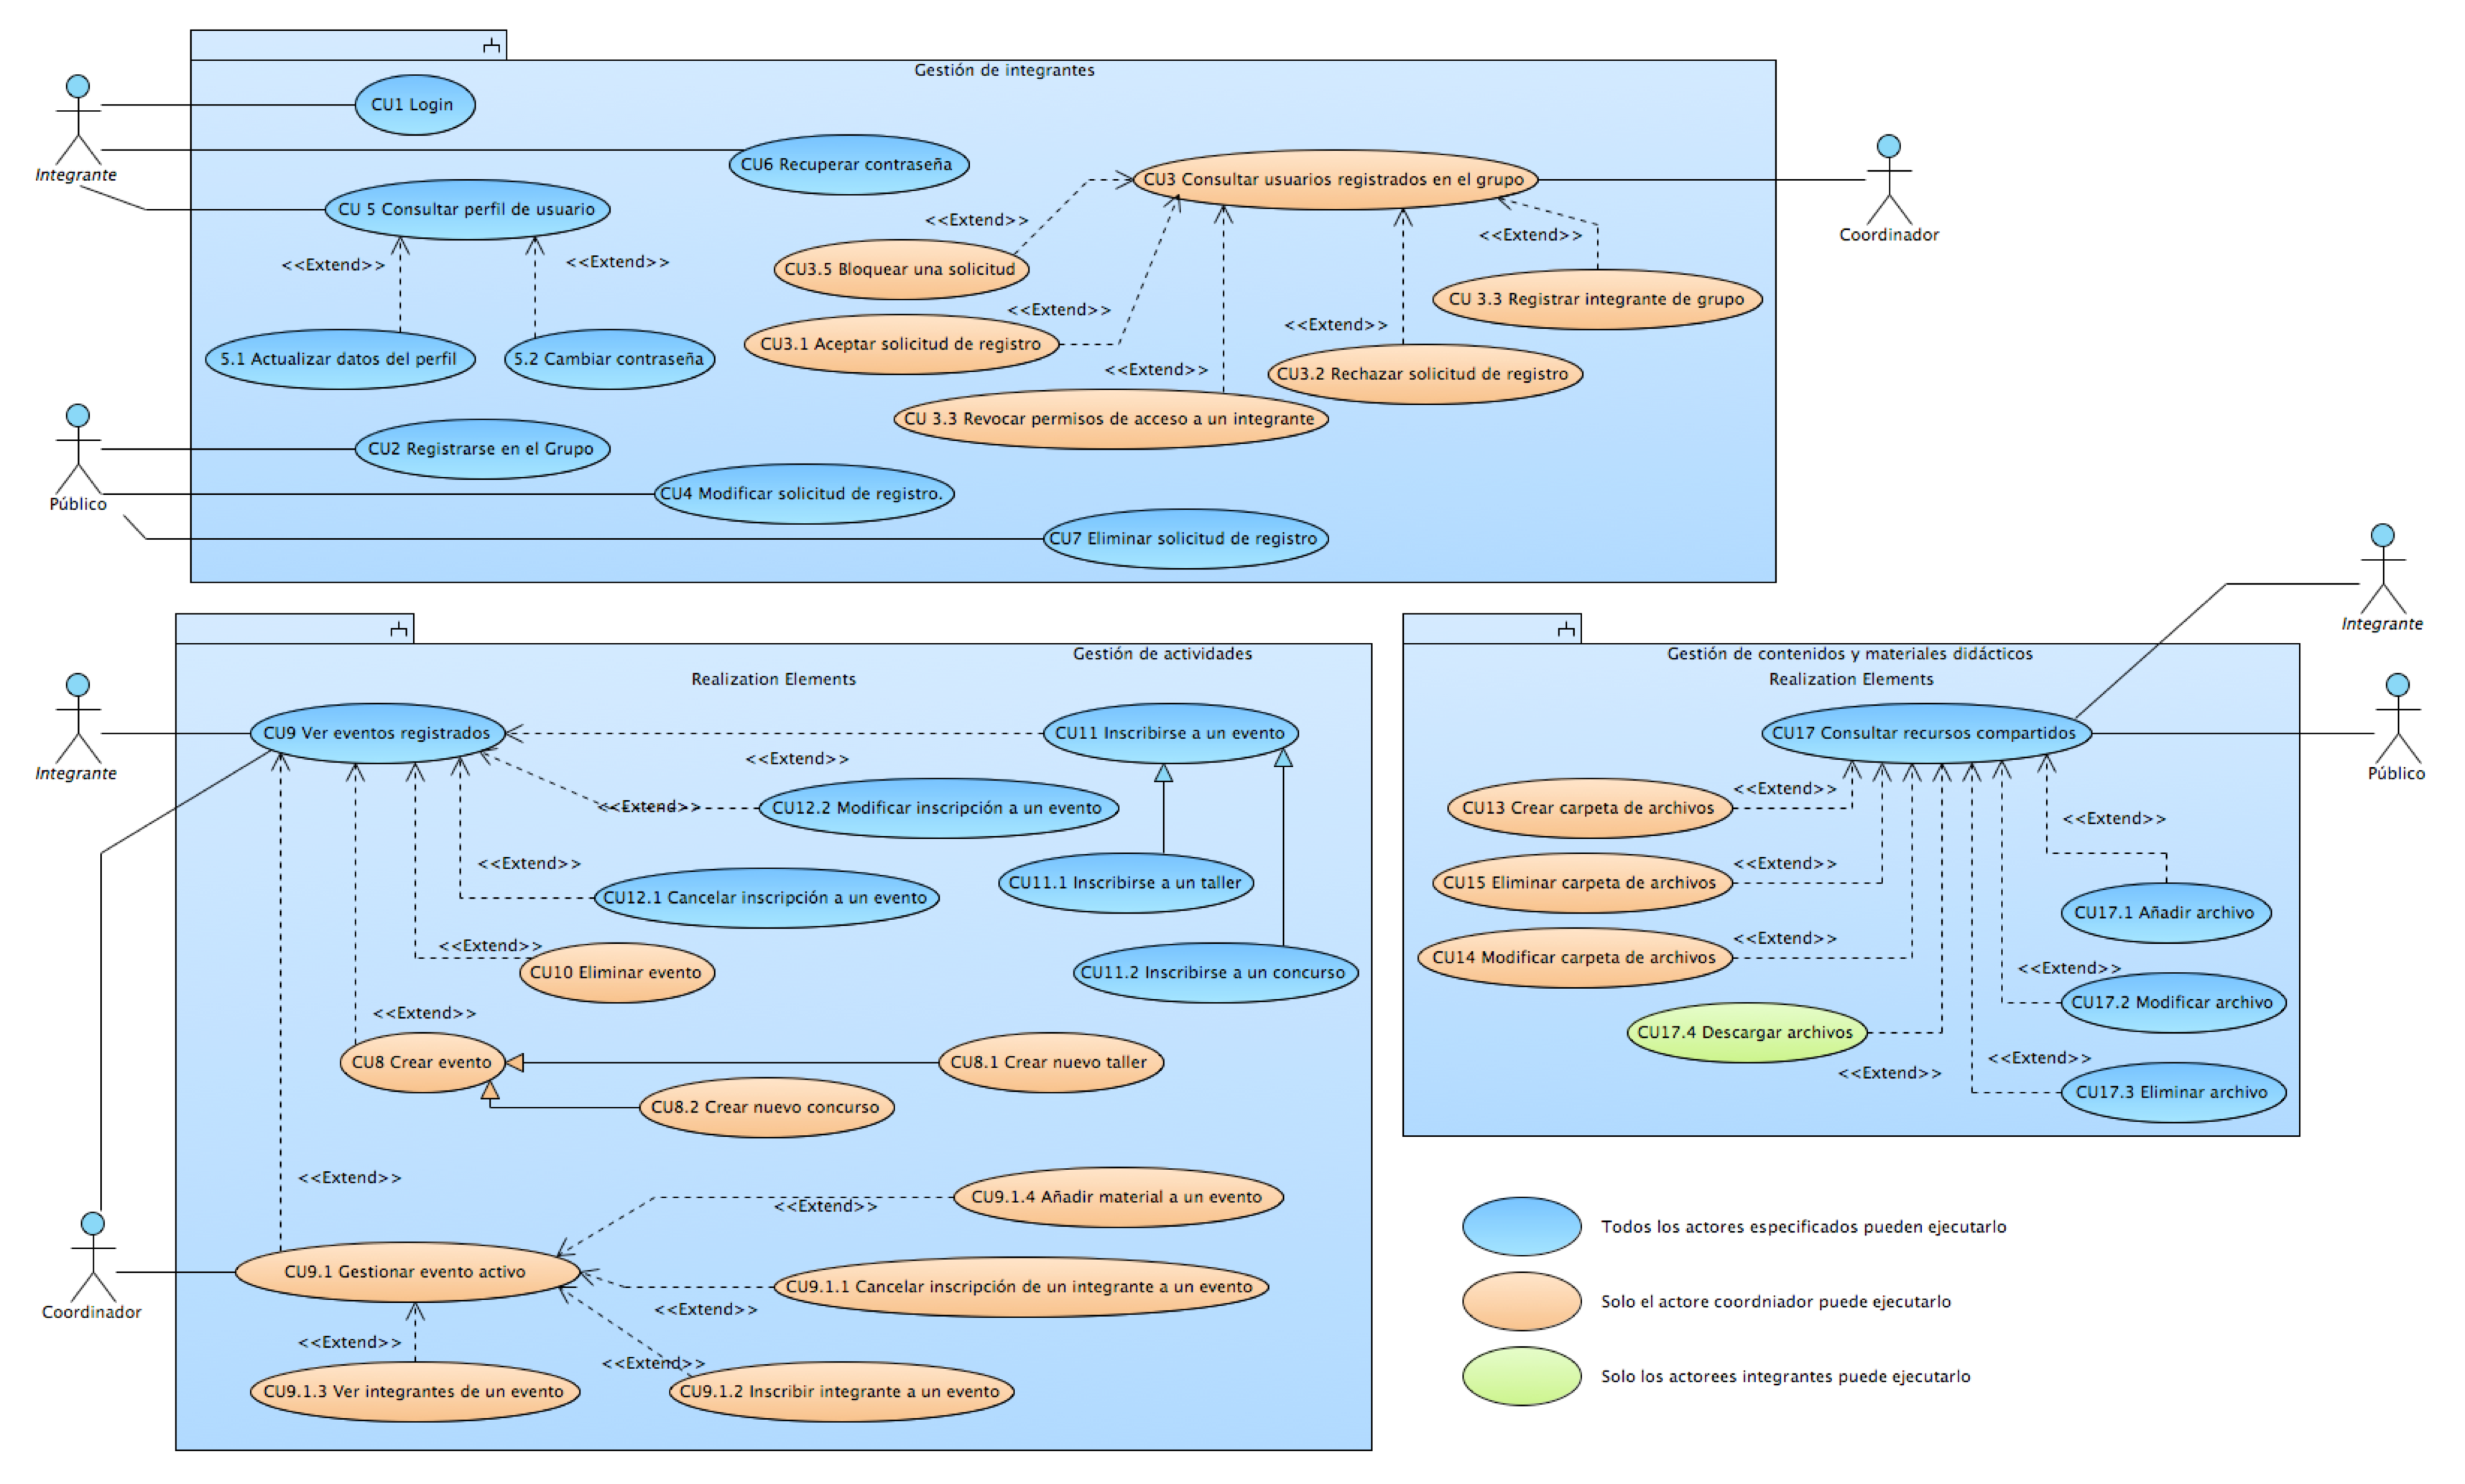
\includegraphics[angle=90, width=.7\textwidth]{images/casosDeUsoDetalle}
		\caption{Diagrama detallado del sistema.}
		\label{fig:casosDeUsoDetalle}
	\end{center}
\end{figure}

%---------------------------------------------------------
\section{Descripción de actores}

%---------------------------------------------------------
\begin{Usuario}{\hypertarget{getenteOperaciones}{\subsection{Gerente de Operaciones}}}{
	Es el encargado de todas las operaciones de la empresa y está por encima de los ejecutivos de producción y de ventas principalmente.
}
    \item[Responsabilidades:] \cdtEmpty
    \begin{itemize}
		\item Supervisar la operación.
		\item Plantear y supervisar el logro de las metas de la empresa y su crecimiento económico.
		\item ...
    \end{itemize}

	\item[Perfil:] \cdtEmpty
    \begin{itemize}
		\item Amplia experiencia en el ramo.
		\item Licenciatura como mínimo.
		\item ...
    \end{itemize}
\end{Usuario}

A continuación se detallan los casos de uso.

%---------------------------------------------------------
% CASOS DE USO

% \IUref{IUAdmPS}{Administrar Planta de Selección}
% \IUref{IUModPS}{Modificar Planta de Selección}
% \IUref{IUEliPS}{Eliminar Planta de Selección}

% 


% Copie este bloque por cada caso de uso:
%-------------------------------------- COMIENZA descripción del caso de uso.

%\begin{UseCase}[archivo de imágen]{UCX}{Nombre del Caso de uso}{
%--------------------------------------
	\begin{UseCase}{CU17}{Inscribir a Seminario}{
		Ayudar a que los Estudiantes que están por terminar la carrera se puedan inscribir en un Seminario de titulación.
	}
		\UCitem{Versión}{\color{Gray}0.1}
		\UCitem{Autor}{\color{Gray}David Ortega Pacheco}
		\UCitem{Supervisa}{\color{Gray}Ulises Vélez Saldaña.}
		\UCitem{Actor}{\hyperlink{Alumno}{Alumno}}
		\UCitem{Propósito}{Que el Estudiante se pueda inscribir a un seminario de titulación.}
		\UCitem{Entradas}{Número de boleta, Contraseña y Seminario.}
		\UCitem{Origen}{Teclado}
		\UCitem{Salidas}{Seminarios registrados, horario actual del Estudiante, desglose del monto a pagar por la inscripción, recibo de pago y comprobante de inscripción.}
		\UCitem{Destino}{Pantalla e impresora para recibo de pago y comprobante de inscripción}
		\UCitem{Precondiciones}{El estudiante debe estar registrado en la universidad.}
		\UCitem{Postcondiciones}{El estudiante quedará inscrito en el Seminario seleccionado si es elegible y hay cupo en el Seminario en cuestión.}
		\UCitem{Errores}{}
		\UCitem{Tipo}{Caso de uso primario}
		\UCitem{Observaciones}{}
	\end{UseCase}
%--------------------------------------
	\begin{UCtrayectoria}{Principal}
		\UCpaso[\UCactor] Introduce su Número de Boleta y Contraseña en el sistema vía la  \IUref{IU23}{Pantalla de Control de Acceso}\label{CU17Login}.
		\UCpaso[\UCactor] Confirma la operación presionando el botón \IUbutton{Entrar}.
		\UCpaso Verifica que el Estudiante sea elegible para inscribirse al Seminario con base en la regla \BRref{BR129}{Determinar si un Estudiante puede inscribir Seminario.} \Trayref{A}.
		\UCpaso Despliega la \IUref{IU32}{Pantalla de Selección de Seminario} con la lista de Seminarios Disponibles.
		\UCpaso[\UCactor] Selecciona el Seminario en el que desea inscribirse \Trayref{B}\label{CU17SeleccionarSeminario}.
		\UCpaso Verifica que el Estudiante sea elegible para inscribirse al seminario seleccionado con base en la regla \BRref{BR130}{Determinar si un Estudiante puede inscribirse en un Seminario} \Trayref{C}.
		\UCpaso Verifica que el horario del Seminario concuerde con el horario del Estudiante con base en la regla \BRref{BR143}{Validar el horario del estudiante} \Trayref{D}.
		\UCpaso Calcula el costo del Seminario basado en el costo publicado en el catálogo de cursos, los costos aplicables al alumno y los impuestos aplicables, con base en las reglas \BRref{BR180}{Calcular costos del Estudiante} y \BRref{BR45}{Calcular impuestos por seminario}.
		\UCpaso Despliega el desglose de costos en la \IUref{IU33}{Pantalla Mostrar costos por seminario}.
		\UCpaso Pide al Estudiante que confirme la inscripción alSeminario.
		\UCpaso[\UCactor] Confirma la inscripción al Seminario.
		\UCpaso Inscribe al Estudiante en el Seminario seleccionado.
		\UCpaso Informa que la inscripción se realizó exitosamente vía la \IUref{UI88}{Pantalla de resumen de inscripción al Seminario}. 
		\UCpaso Imprime el recibo de pago con base en la regla \BRref{BR100}{Recibo del Estudiante por inscripción a Seminario.}.
		\UCpaso Pregunta al estudiante si desea imprimir un comprobante de la inscripción.
		\UCpaso[\UCactor] Indica que desea imprimir el comprobante de la inscripción.
		\UCpaso Imprime el comprobante de la inscripción \IUref{IU189}{Reporte de inscripción a Seminario}.		
	\end{UCtrayectoria}

%--------------------------------------		
		\begin{UCtrayectoriaA}{A}{El Estudiante no puede inscribir un Seminario}
			\UCpaso Muestra el Mensaje {\bf MSG1-}``El Estudiante [{\em Número de Boleta}] aun no puede inscribirse al seminario.''.
			\UCpaso[\UCactor] Oprime el botón \IUbutton{Aceptar}.
			\UCpaso[] Termina el caso de uso.
		\end{UCtrayectoriaA}
		
%--------------------------------------
		\begin{UCtrayectoriaA}{B}{El Estudiante abandona la operación}
			\UCpaso El Estudiante revisa la lista de Seminarios y no encuentra el Seminario que desea.
			\UCpaso[\UCactor] Oprime el botón \IUbutton{Salir}.
			\UCpaso Cierra la sesión del usuario.
			\UCpaso Continua en el paso \ref{CU17Login} del \UCref{CU17}.
		\end{UCtrayectoriaA}

%--------------------------------------
		\begin{UCtrayectoriaA}{C}{El estudiante no cumple con los prerrequicitos}
			\UCpaso Muestra el Mensaje {\bf MSG2-}``El Estudiante [{\em Número de Boleta}] no cumple con los requisitos para inscribirse al Seminario [{\em Nombre del Seminario seleccionado}].''.
			\UCpaso Muestra los requisitos que el Seminario seleccionado solicita.
			\UCpaso Continúa en el paso \ref{CU17SeleccionarSeminario} del \UCref{CU17}.
		\end{UCtrayectoriaA}

%--------------------------------------
		\begin{UCtrayectoriaA}{D}{El horario es incompatible.}
			\UCpaso Muestra el Mensaje {\bf MSG3-}``El horario del [{\em Nombre del Seminario seleccionado}] no es compatible con el horario del curso [{\em Nombre de la materia y grupo del curso con el que choca el horario}].''.
			\UCpaso Continúa en el paso \ref{CU17SeleccionarSeminario} del \UCref{CU17}.
		\end{UCtrayectoriaA}

%--------------------------------------
% Puntos de extensión
\subsection{Puntos de extensión}
\UCExtenssionPoint{
	% Cuando:
	Desea conocer las materias cursadas.
}{
	% Durante la región:
	Del paso 4 al paso 9.
}{
	% Casos de uso a los que extiende:
	\hyperlink{CU3.4}{CU3.4 Consultar historial académico}.
}
		
		
		
%-------------------------------------- TERMINA descripción del caso de uso.





%=========================================================
%=========================================================
\chapter{Modelo de la interacción}	
\label{cap:modInteraccion}

	Este capítulo describe ...

\section{Modelo de navegación}

	La navegación entre pantallas se muestra en la figura~\ref{fig:mapa}. en el se explica ...\\

\begin{figure}[htbp]
	\begin{center}
		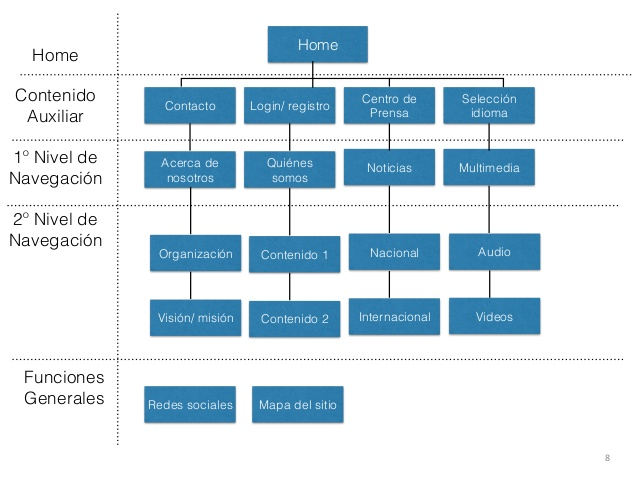
\includegraphics[width=.7\textwidth]{images/mapa}
		\caption{mapa}
		\label{fig:mapa}
	\end{center}
\end{figure}

%--------------------------------------
\section{IU23 Pantalla de Control de Acceso}

\subsection{Objetivo}
	Controlar el acceso al sistema mediante una contraseña a fin de que cada usuario acceda solo a las operaciones permitidas para su perfil.

\subsection{Diseño}
	Esta pantalla \IUref{IU23}{Pantalla de Control de Acceso} (ver figura~\ref{IU23}) aparece al iniciar el sistema. Para ingresar al mismo se debe escribir el Número de Boleta del estudiante y la contraseña de acceso. 

\IUfig[.5]{Login}{IU23}{Pantalla de Control de Acceso.}

\subsection{Salidas}

	Ninguna.

\subsection{Entradas}
Número de Boleta y Contraseña del Estudiante.

\subsection{Comandos}
\begin{itemize}
	\item \IUbutton{Entrar}: Verifica que el Estudiante se encuentre registrado y la contraseña sea la correcta. Si la verificación es correcta, se muestra la \IUref{UI32}{Pantalla de Selección de Seminario}.
	\item \IUbutton{Ayuda}: Muestra la ayuda de esta pantalla \IUref{IU50}{Pantalla de Ayuda}.
\end{itemize}

\subsection{Mensajes}

\begin{Citemize}
	\item Error al verificar los datos de acceso, vuelva a intentarlo.
\end{Citemize}





\end{document}
